\section{InferSpark Overview}
\label{sec:framework}

%\begin{figure*}[th]
%	\centering
%	\includegraphics[width=1.6\columnwidth]{figs/workflow2.eps}
%	\caption{InferSpark Architecture}
%	\label{fig:workflow}
%\end{figure*}

%\KZ{My general feeling is that the running example is not made full use of.
%The discussion should be tightly coupled to the running example. E.g., when
%we talk about schedule, just present the schedule for the two coins.
%Some of the stuff here should go into implementation section.}

%The overall architecture of InferSpark is shown in \figref{fig:workflow}.  
An InferSpark program is a mix of Bayesian network model definition and normal
user code. In the following, we will illustrate the use of InferSpark through a simple
Bayesian network model called two-coin.  We show how to encode the model, instantiate
the model with input data, and infer model parameters from the data.
Finally, we give the formal syntax of InferSpark.

%Note that we currently hard-code the VMP algorithm into CodeGen module of
%InferSpark, which only supports certain exponential-conjugate Bayesian
%networks. We plan to implement other inference algorithms such as Belief
%Propagation, Gibbs Sampling, etc. to handle other common types of Bayesian
%networks.

%InferSpark analyzes the Bayesian network defined by a special 
%scala-like program and
%automatically transforms the model definition into the GraphX implementation
%of VMP algorithm. After two stages of compilation, the runtime system 
%launches the VMP implementation and returns the inference results 
%through the query API.  
%Next, we describe the key modules in more details with the help of
%some Baysian models. 
%the example of the two-coin model (\figref{fig:two_coin_bn}). 

\subsection{Simple Two-coin Example}

\begin{figure}[th]
	\centering
	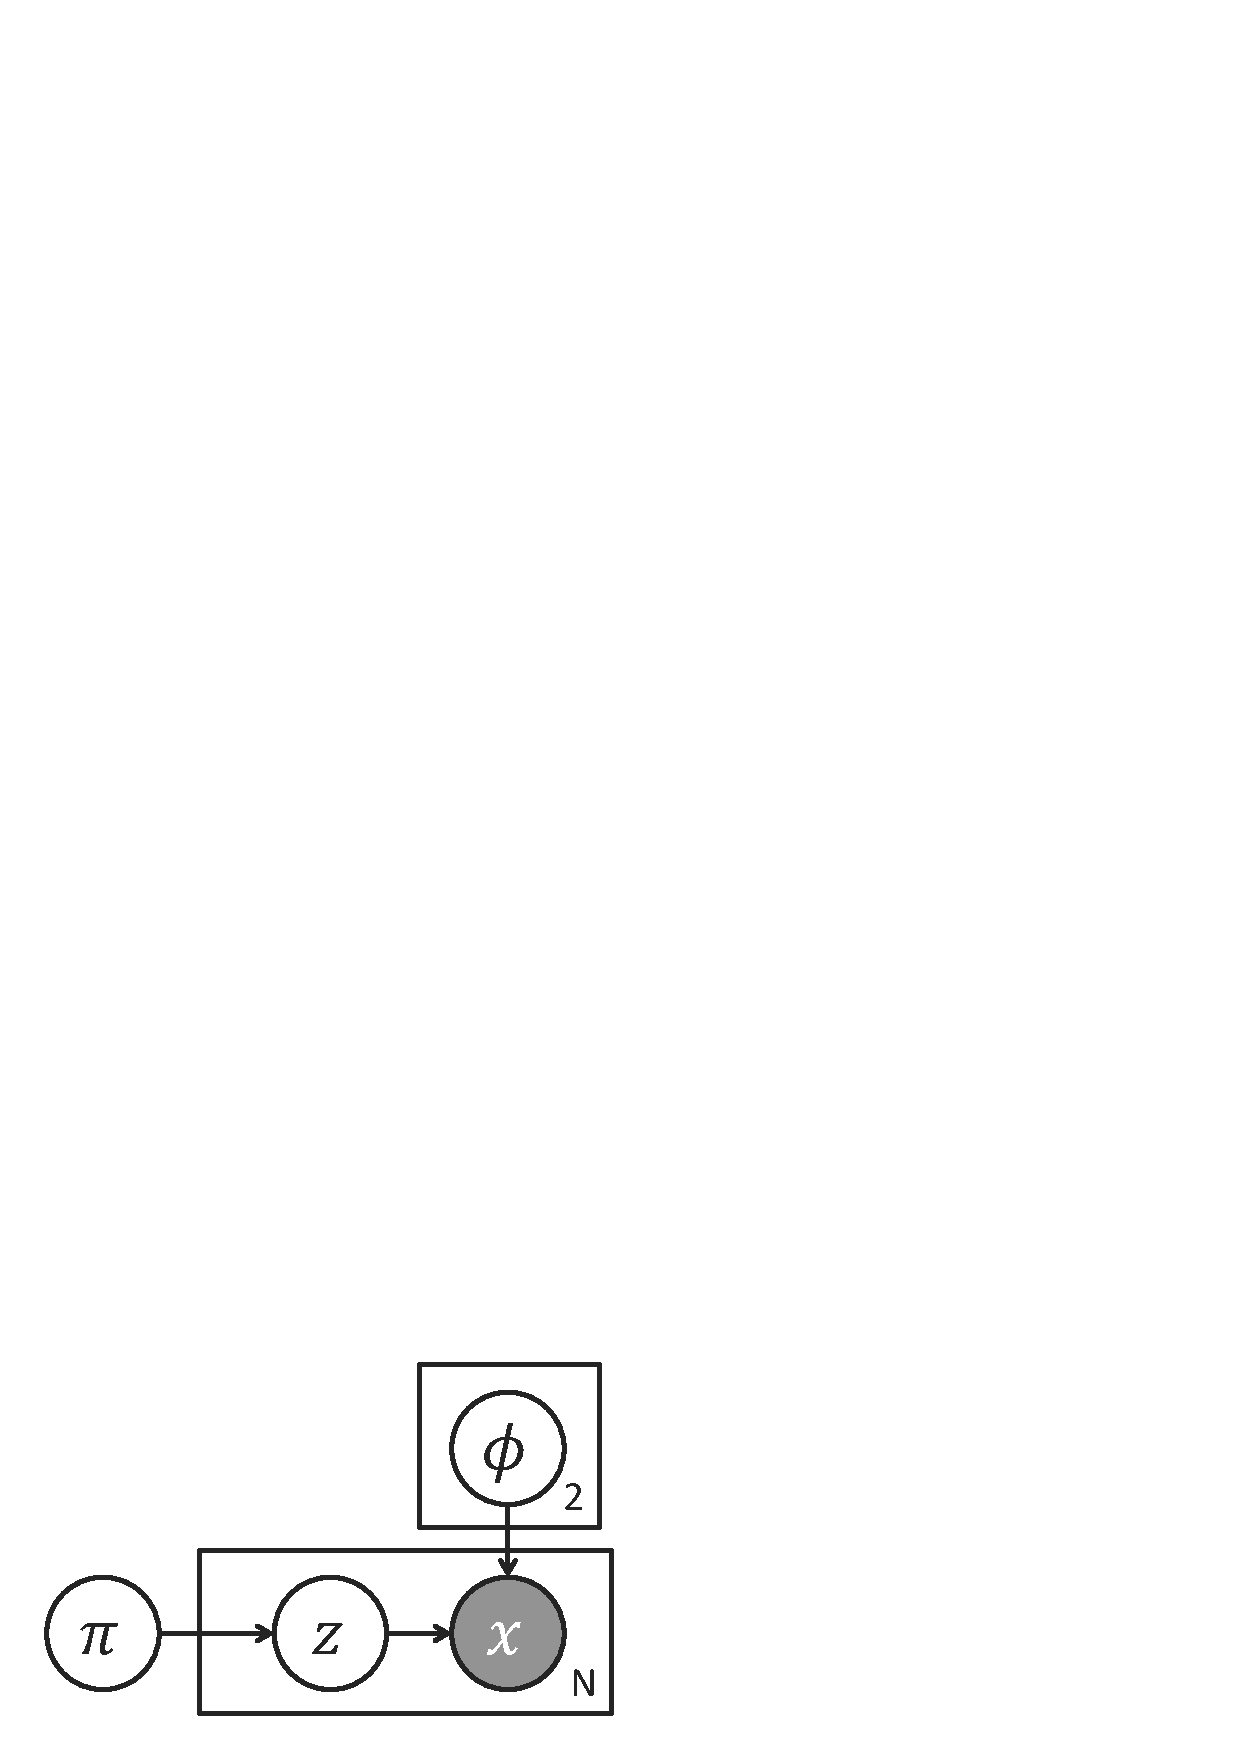
\includegraphics[width=0.25\textwidth]{figs/two_coins_latent}
	\caption{Two-coin Model with Latent Variable}
	\label{fig:two_coins}
\end{figure}
Consider a two-coin model in \figref{fig:two_coins}, where we first decide
which coin to toss, with probability $\pi_1$ to choose coin 1 and
probability $\pi_2$ to choose coin 2 ($\pi_1 = 1 - \pi_2$). 
Latent variable $z$ ranges over coin 1 or coin 2. 
We then toss the chosen coin, which has probability $\phi_i$ to turn up head.
This process is repeated $N$ times. The outcome of the toss are represented by observable
variable $x$. The two-coin model is a {\em mixture model}, which represents the
mixture of multiple sub-populations. Each such sub-population, in this case
$\phi_1$ and $\phi_2$, have their own distributions,
while the observation can only be obtained on the overall population, that is
the number of heads after $N$ tosses.


\subsection{Model Definition}
\begin{figure}[th]
\begin{lstlisting}
@Model class TwoCoins(alpha: Double, beta: Double) {
	val pi = Beta(alpha)
	val phi = (0L until 2L).map(_ => Beta(beta))
	val z = ?.map(_ => Categorical(pi))
	val x = z.map(z => Categorical(phi(z)))
}
object Main {
	def main() {
		val xdata: RDD[Long] = /* load (observed) data */
		val m = new TwoCoins(1.0, 1.0)
		m.x.observe(xdata)
		m.inferVMP(steps=20) /* alternative is inferGS */
		val postPhi: VertexRDD[BetaResult] = m.phi.getResult()
		/* postprocess */
		...
	}
}
\end{lstlisting}
\caption{The InferSpark Description of Two-coin Model}
\label{fig:two_coins_modeldef}
\end{figure}

%Apart from ordinary scala code, the input program of InferSpark contains the
%statistical model definitions. The syntax of the model definition extends
%from the scala syntax.  
\figref{fig:two_coins_modeldef} shows a fragment of InferSpark program implementing
the two-coin model. 
The model definition starts with ``{\sf @Model}'' annotation. 
The rest is similar to a class definition in
scala. The model parameters (``{\sf alpha}'' and ``{\sf beta}'') are constants to the
model. In the model body, only a sequence of value definitions are allowed,
each defining a random variable instead of a normal deterministic variable. 
The use of ``{\sf val}'' instead of ``{\sf var}'' in the syntax 
implies the conditional dependencies between random variables are fixed 
once defined. For example, line 2 defines the random variable 
$\pi$ having a symmetric Beta prior
$\mathrm{Beta}(\alpha, \alpha)$.

InferSpark model uses ``Range'' class in Scala to represent plates. Line 3
defines a plate of size 2 with the probabilities of seeing head in the 
two coins. The ``?'' is a special type of ``Range'' representing 
a plate of unknown size at the time of model definition. 
In this case, the exact size of the plate will be provided or inferred
from observed variables at run time.  When a random variable is
defined by mapping from a plate of other random variables, 
the new random variable is in the same plate as the others.  
For example, line 5 defines the outcomes $x$ as the mapping from $z$ 
to Categorical mixtures, therefore $x$ will be in the same plate as
$z$. Since the size of the plate surrounding $x$ and $z$ is unknown, we need
to specify the size at run time.  We can either explicitly set the length of
the ``?'' or let InferSpark set that based on the number of observed outcomes
$x$ (line 11).

At the first glance, ``?'' seems redundant since it can be replaced by a
model parameter $N$ denoting the size of the plate.  However, ``?'' becomes
more useful when there are nested plates. In the two-coin model, suppose
after we choose one coin, we toss it multiple times. 
%\figref{fig:two_coins_nestedplates} shows this scenario.
Then the outcomes $x$ are in two nested plates where the inner plate is
repeated $N$ times, and each instance may have
a different size $M_i$. Using the ``?'' syntax
for the inner plate, we simply change line 5 to

{\small\begin{verbatim}
	val x = z.map(z => ?.map(_ => Categorical(phi(z))))	
\end{verbatim}
}


\subsection{Rest of the Program}
%InferSpark finally compiles the VMP algorithm into a separate GraphX
%program and submit it to the Spark master. The user can specify how many
%iterations to run. 
The model definition needs to be instantiated with observed data and
other meta data at runtime (e.g., the outcomes $x$, the number of coin flippings
and the model parameters $\alpha$ and $\beta$). These are done in the
remaining user Scala code, defined  as ``{\sf object Main}'' in
\figref{fig:two_coins_modeldef}.

In Line 9, {\sf xdata} is defined as a Spark Vertex RDD, which stores the information of 
observed data. 
Then an instance of the model is created via the constructor invocation (e.g.
``{\sf val m = new TwoCoin(1.0, 1.0)}'' on line 10. 
The constructor call provides
the missing constants in the prior distributions of $\pi$ and $\phi$.
For each random variable defined in the model definition,
there is an interface field with the
same name in the constructed object. 

Observed values are provided to InferSpark
by calling the ``{\sf observe}'' (line 11) API on the field.
There, the user provides an RDD of observed outcomes ``{\sf xdata}'' to InferSpark by calling
``{\sf m.x.observe(xdata)}''. The  {\sf observe} API also triggers
the calculation of unknown plate sizes.
In this case, the size of plate surrounding $z$ and $x$ is
automatically calculated by counting the number of elements in the RDD.


Line 12 does the actual inference on the model.
Currently InferSpark provides two inference algorithms: VMP and Gibbs sampling. 
They can be invoked by either ``{\sf inferVMP}'' or ``{\sf inferGS}'' API. The number
of steps configures the number of iterations to be run by each of these algorithms.
After the call to the infer API, unknown parameters in the model will be
inferred and persisted in the object {\sf m}.

The inference results can be queried through the ``{\sf getResult}''
API on fields in the model instance that retrieves a VertexRDD of approximate
marginal posterior distribution of the corresponding random variable. For
example, in Line 13 of \figref{fig:two_coins_modeldef}, ``{\sf m.phi.getResult()}'' 
returns a VertexRDD of two Dirichlet distributions. 
The user can also call ``{\sf lowerBound}'' 
on the model instance to get the evidence lower bound (ELBO) of the result, 
which is higher when the KL divergence between the approximate posterior 
distribution and the true posterior is smaller. 

\begin{figure}[h]
\centering
\begin{lstlisting}
var lastL: Double = 0
m.infer(20, { m =>
	if ((m.roundNo > 1) || 
		(Math.abs(m.lowerBound - lastL) < 
		   Math.abs(0.001 * lastL))) {
		false
	} else {
		lastL = m.lowerBound
		true	
	}
})
\end{lstlisting}
\caption{Using Callback function in ``infer'' API}
\label{fig:two_coins_callback}
\end{figure}

The user can also provide a callback function that will be called after
initialization and each iteration. In the function, the user can write
progress reporting code based on the inference result so far. 
For example, this function may return {\em false} whenever
the ELBO improvement is smaller than a threshold 
(see \figref{fig:two_coins_callback}) indicating the result is good enough 
and the inference should be terminated. 

%With all the information collected and calculated in previous steps,
%implementation of the inference algorithm as a GraphX program is generated,
%compiled and then executed. User can retrieve the posterior distributions as
%VertexRDDs through API calls.

\subsection{InferSpark Syntax}

%In this offline compilation stage, the model definition is first transformed
%into a Bayesian network.  We use the macro annotation, a compile-time meta-programming
%facility of Scala reflection. After the parser phase, the class annotated with ``{\sf @Model}'' 
%annotation is passed from the compiler to the transform method of
%InferSpark. InferSpark treats the class passed to it as model definition and
%transforms it into a Bayesian network.

\begin{figure}[!h]
\centering
\small
	\begin{tabular}{lrl}
		ModelDef		& ::= & `@Model' `class' id \\
					&     &`(' ClassParamsOpt `)' `\{' Stmts `\}' \\
		ClassParamsOpt	& ::= & `' /* Empty */ \\
						&	| &	ClassParams \\
		ClassParams		& ::= & ClassParam  [`,' ClassParams] \\
		ClassParam		& ::= & id `:' Type \\
		Type			& ::= & `Long' | `Double' \\
		Stmts			& ::= & Stmt [[semi] Stmts]\\
		Stmt			& ::= & `val' id = Expr \\
		Expr			& ::= & `\{' [Stmts [semi]] Expr `\}' \\
						&	| & DExpr	\\
						&   | & RVExpr \\
						&	| & PlateExpr \\
						&	| & Expr `.' `map' `(' id => Expr `)'\\
		DExpr			& ::= & Literal	\\
						&   | & id \\
						&   | & DExpr (`+' | `-' | `*' | `/') DExpr \\
						&   | & (`+' | `-') DExpr	\\
		RVExpr			& ::= & `Dirichlet' `(' DExpr `,' DExpr `)' \\
						&   | & `Beta' `(' DExpr `)' \\
						&   | & `Categorical' `(' Expr `)' \\
						&   | & `Gaussian' `(' DExpr, DExpr `)' \\
						&   | & RVExpr RVArgList	\\
						&   | & id	\\
		RVArgList		& ::= & `(' RVExpr `)' [ RVArgList ] \\
		PlateExpr		& ::= & DExpr `until' DExpr	\\ 
						&   | & DExpr `to' DExpr	\\
						&	| & `?' \\
						&	| & id
	\end{tabular}
\caption{InferSpark model definition syntax}
\label{fig:inferspark_syntax}
\end{figure}

\figref{fig:inferspark_syntax} shows the formal definitions
of syntax of InferSpark model definition. 
The expressions in a model definition is divided into 3
categories: deterministic expressions (DExpr), random variable expressions
(RVExpr) and plate expressions(PlateExpr). 
The deterministic expressions include literals, 
class parameters and their arithmetic operations. The random
variable expressions define random variables or plates of random variables.
The plate expressions define plate of known size or unknown size. The random
variables defined by an expression can be binded to an identifier by the value
definition. It is also possible for a random variable to be bound to multiple
or no identifiers. To uniquely represent the random variables, we assign
internal names to them instead of using the identifiers.

